\chapter{Background \& Related Work}
\label{ch:background}
In this chapter we will give a introduction into the different fields touched by our research.
Related work is mentioned primarily in section~\ref{ch:background:se:graphDatabaseBenchmarks} as it covers the different benchmarks and their findings.

\section{Graphs}
\label{ch:background:se:graphs}
A graph as the literature tells us~\cite[89]{Worsch2011} is a tuple of sets $ G = (V, E) $ with $ E \subseteq V \times V $.
Elements of $ V $ are called vertices and elements of $ E $ are called edges.
The set of vertices has to be not empty, but the edge set can be.
In this thesis we are focusing on directed graphs only,
although some graph databases are capable of handling undirected graphs too not all are.
Also there would be no benefit in using undirected edges since our model also uses directed edges.
In general graphs can have labels or weights on their edges as stated in~\cite[99]{Worsch2011}.
For our purposes we will use labels on the vertices and edges to ease the understanding of our data structure.
In section~\ref{ch:background:se:graphDatabases} we will give reasons why having labels on the graph components is useful.

Figure~\ref{fig:simpleGraph} shows an example of a directed graph with labels on its vertices.
An equivalent representation of that graph would be
\begin{equation}
  \begin{aligned}
    V &= \{1, 2, 3\} \\
    E &= \{(1, 2), (1, 3), (2, 3), (3, 2)\}.
  \end{aligned}
\end{equation}

\begin{figure}[h]
  \centering
  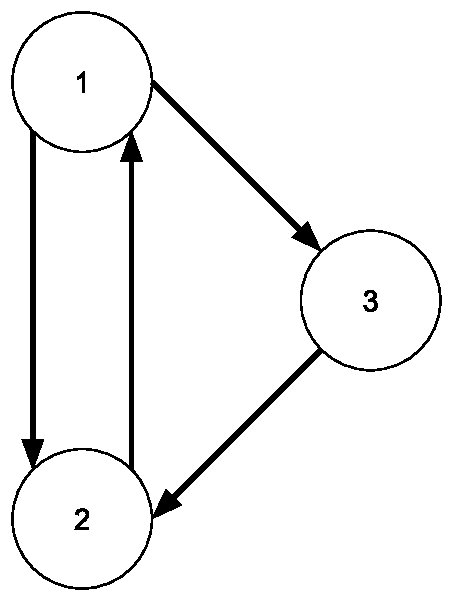
\includegraphics[width=\textwidth/4]{images/simpleGraph}
  \caption{A directed graph with three labeled vertices and four edges.}
  \label{fig:simpleGraph}
\end{figure}

\subsection{Trees}
\todo{Explain tree graphs shortly.}

\section{Industrial Data}
\label{ch:background:se:industrialData}
Under the term "industrial data" we understand data that is produced by machines during the production.
That could be the current settings of the machine,
temperatures or tolerances measured during processing or what product is currently worked on.
In chapter~\ref{ch:analysis:se:data} the possible structure of this data is analysed.

As there is no publicly available information about how industrial data should look like we will use the example given by our partners at SICK AG~\cite{SICK} as an inspiration for our test data.

Listing~\ref{lst:exampleData} shows the graph excerpt of our given example.

\begin{lstlisting}[language={XML},label={lst:exampleData},caption={An excerpt showing the observation of components.}]
"@graph": [
  {
    "@id": "http://localhost:3000/observations/185",
    "@type": "ssn:Observation",
    "featureOfInterest": "aoi:Feature",
    "observationSamplingTime": "2016-05-18T12:55:27.954Z",
    "observedProperty": [
      "aoi:twisting",
      "aoi:y-shift",
      "aoi:x-shift"
    ],
    "observationResult": "http://localhost:3000/observations/185/sensor-output",
    "observationResultTime": "2016-05-18T12:55:27.954Z",
    "observedBy": "http://localhost:3001/AOI_SMD407",
    "dataClass": "Testdata"
  },
  {
    "@id": "http://localhost:3000/observations/185/sensor-output",
    "@type": "ssn:SensorOutput",
    "isProducedBy": "http://localhost:3001/equipment/AOI_SMD407",
    "hasValue": "http://localhost:3000/observations/185/result"
  },
  {
    "@id": "http://localhost:3000/observations/185/result",
    "@type": "ssn:ObservationValue, shopfloor:Panel",
    "orderNo":"http://localhost:3000/order#0",
    "partNr": "http://localhost:3000/part#2060817",
    "hasPart": "http://localhost:3000/observations/185/board#3827581",
    "startTime": "2016-05-18T12:55:27.954Z",
    "endTime": "2016-05-18T12:56:27.954Z"
  },
  {
    "@id": "http://localhost:3000/observations/185/board#3827581",
    "@type": "shopfloor:Board",
    "hasPart": ["http://localhost:3000/observations/185/component#C1-1","http://localhost:3000/observations/185/component#C2-1"],
    "boardUID":"3827581",
    "isBadBoard": false
  },
  {
    "@id": "http://localhost:3000/observations/185/component#C1-1",
    "@type": "shopfloor:Component",
    "componentType": "C0603",
    "position":0,
    "testFeature":[
      {
        "@id": "http://localhost:3000/observations/185/component#C0603-MENI-901-TWISTING",
        "feature": "aoi:twisting1",
        "analysisMode": [
          {"@id": "http://localhost:3000/observations/185/AnalysisMode#C0603-MENI-901-TWISTING",
            "windowNumber": "901",
            "featureFlag": "0",
            "mode":"MENI"
          }
        ],
        "hasValue": {
          "@type": "xsd:integer",
          "@value": "10"
        }

      },
      {
        "@id": "http://localhost:3000/observations/185/component#C0603-MENI-901-Y-Shift",
        "feature": "aoi:y-shift1",
        "analysisMode": [
          {"@id": "http://localhost:3000/observations/185/AnalysisMode#C0603-MENI-901-Y-Shift",
            "windowNumber": "901",
            "featureFlag": "0",
            "mode":"MENI"
          }
        ],
        "hasValue": {
          "@type": "xsd:integer",
          "@value": "-17"
        }
      },
      {
        "@id": "http://localhost:3000/observations/185/component#C0603-MENI-901-X-Shift",
        "feature": "aoi:x-shift1",
        "analysisMode": [
          {"@id": "http://localhost:3000/observations/185/AnalysisMode#C0603-MENI-901-X-Shift",
            "windowNumber": "901",
            "featureFlag": "0",
            "mode":"MENI"
          }
        ],
        "hasValue": {
          "@type": "xsd:integer",
          "@value": "20"
        }
      }
    ]
  },
  {
    "@id": "http://localhost:3000/observations/185/component#C2-1",
    "@type": "aoi:Component",
    "componentType": "C0603",
    "position":0,
    "testFeature":[
      {
        "@id": "http://localhost:3000/observations/185/component#C0603-MENI-901-TWISTING",
        "feature": "aoi:twisting1",
        "analysisMode": [
          {"@id": "http://localhost:3000/observations/185/AnalysisMode#C0603-MENI-901-TWISTING",
            "windowNumber": "901",
            "featureFlag": "0",
            "mode":"MENI"
          }
        ],
        "hasValue": {
          "@type": "xsd:integer",
          "@value": "12"
        }
      },
      {
        "@id": "http://localhost:3000/observations/185/component#C0603-MENI-901-Y-Shift",
        "feature": "aoi:y-shift1",
        "analysisMode": [
          {"@id": "http://localhost:3000/observations/185/AnalysisMode#C0603-MENI-901-Y-Shift",
            "windowNumber": "901",
            "featureFlag": "0",
            "mode":"MENI"
          }
        ],
        "hasValue": {
          "@type": "xsd:integer",
          "@value": "14"
        }
      },
      {
        "@id": "http://localhost:3000/observations/185/component#C0603-MENI-901-X-Shift",
        "feature": "aoi:x-shift1",
        "analysisMode": [
          {"@id": "http://localhost:3000/observations/185/AnalysisMode#C0603-MENI-901-X-Shift",
            "windowNumber": "901",
            "featureFlag": "0",
            "mode":"MENI"
          }
        ],
        "hasValue": {
          "@type": "xsd:integer",
          "@value": "11"
        }
      }
    ]
  }
]
\end{lstlisting}

In figure~\ref{fig:exampleData} the provided example is visualised partially,
it shows the observation of a product.

\begin{figure}
  \centering
  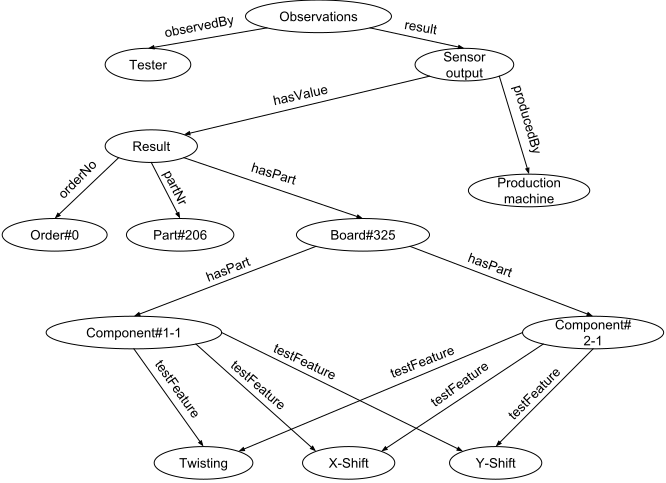
\includegraphics[width=\textwidth]{images/exampleGraph}
  \caption{An example graph representing the observation of test features in the components of a board.}
  \label{fig:exampleData}
\end{figure}

\section{Graph Databases}
\label{ch:background:se:graphDatabases}
\todo{Write about available versions of the databases}
There is a variety of database types available the main categories are SQL and NoSQL databases.
A short description of SQL databases would be
\blockquote[\cite{ChuaHock-Chuan}]{A relational database organizes data in tables (or relations).
A table is made up of rows and columns.
A row is also called a record (or tuple).
A column is also called a field (or attribute).
A database table is similar to a spreadsheet.}

NoSQL databases on the other hand are able to store any kind of data in any record,
they don't rely on a specified schema.
Also they are able to scale horizontally for the cost of consistency.~\cite{Yegulalp2017}

Graph databases are a type of NoSQL databases.
They use graph theory to store their data as described in~\ref{ch:background:se:graphs} with vertices and edges.
Every vertex has a unique identifier (id) in the database,
the edges coming from or going to that vertex and it can have properties assigned to it as key/value pairs.
Edges also have a unique id,
a start and end vertex and properties just as vertices.~\cite{Rouse2016}

The labels mentioned at the end of section~\ref{ch:background:se:graphs} can be seen as the properties assigned to a vertex or edge.
To map a production line in which the elements like machines and products might have their own real world ids these properties can be used to store these real world ids as a key/value pair.
Later a particular machine for example can be looked up by its id.
That is critical to find the data stored in the database.

In the following subsections~\ref{ch:background:se:rdfTriplestores} through~\ref{ch:background:se:graphStores} we will discuss the different types of graph databases and give examples of real databases which operate by that type.
All databases used in this thesis support the ACID\footnote{short for atomicity, consistency, isolation, durability. It should guarantee data validity.} principle with transactions to ensure data consistency.

\subsection{RDF/Triplestores}
\label{ch:background:se:rdfTriplestores}
First in our list are RDF stores also known as triple stores.

RDF (Resource Description Framework) is a model for data interchange on the Web.
It is able to merge data even with different schemas, it also support the evolution of a schema over time.
The linking strucutre of the Web is extended by RDF by it using URIs\footnote{abbreviation of Universal Resource Identifier, used to identify abstract of physical resources.~\cite{Berners-Lee2005}} to name relationships and resources connected by those.~\cite[4]{Ontotext2014}

\blockquote[\cite{W3C2014}]{This linking structure forms a directed, labeled graph, where the edges represent the named link between two resources, represented by the graph nodes.
This graph view is the easiest possible mental model for RDF and is often used in easy-to-understand visual explanations.}

Triplestores store semantic facts as subject - predicate - object triples,
also referred to as statements using RDF.
These statements form a network of data,
which can also be seen as a graph.~\cite[4]{Ontotext2014}

\subsubsection{Apache Jena TDB}
\blockquote[\cite{Apache2015}]{Apache Jena (or Jena in short) is a free and open source Java framework for building semantic web and Linked Data applications.
The framework is composed of different APIs interacting together to process RDF data.}

The TDB component in Jena is responsible to store and query RDF data.~\cite{Apache}

In section~\ref{ch:background:se:graphDatabaseBenchmarks} we will discuss recent studies investigating Apache Jena, among others.

\subsection{Document Stores}
As the name suggests the data model of document stores consist of documents which can have fields without depending on a defined schema~\cite{OrientDB}.
Its aggregates data in those documents and transforms them internally into an searchable form~\cite{Techopedia2017}.

\subsubsection{OrientDB}
OrientDB is a mix of a document store and a graph store,
as stated in their manual \textquote[\cite{OrientDB}]{OrientDB is a document-graph database, meaning it has full native graph capabilities coupled with features normally only found in document databases.}
Its designed as a robust, highly scalable database with a wide possible set of use cases.~\cite{OrientDB}

\subsection{Graph Stores}
\label{ch:background:se:graphStores}
Graph stores organise their data as graphs.
References with foreign keys known from relational databases are mapped as relationships in graph databases.
Each node in the database model contains a list of relationship-records to represent their connection to other nodes.~\cite{NeoTechnologyInc.2016}

\subsubsection{Neo4j}
Neo4j is a native graph database and was build as such from the ground up.
In their introduction they say \textquote[\cite{Neo4jInc.}]{The architecture is designed for optimizing fast management, storage, and traversal of nodes and relationships.
In Neo4j, relationships are first class citizens that represent pre-materialized connections between entities.}

\subsubsection{Sparksee}
The user manual describes Sparksee as follows, \textquote[\cite{SparsityTechnologies}]{Sparksee is an embedded graph database management system tightly integrated with the application at code level.}
Sparksee is implemented in C++ but provides a low level Java API.

\section{Graph Database Benchmarks}
\label{ch:background:se:graphDatabaseBenchmarks}
\todo{Add benchmark results}
As the need to compare similar programs exists benchmarks are needed to hand results over certain parameters to aid decision making.
In the field of graph databases that is no different.
There exist multiple benchmarks for graph databases and some are outlined shortly in the following subsections~\ref{ch:background:se:ldbcGraphalytics}~to~\ref{ch:background:se:ycsb}.
In in section~\ref{ch:analysis:se:benchmark} we choose a benchmark for our work.

\subsection{LDBC: Graphalytics}
\label{ch:background:se:ldbcGraphalytics}
Benchmark specifications, practices and results for graph data management systems are established by an industry council called The Linked Data Benchmark Council.
The Graphalytics benchmark facilitates a choke-point design to evaluate the crucial technological challenges present in system design,
one example would be the "large graph memory footprint" as mentioned in~\cite[2]{Capota2015c}.

Graphalytics uses Datagen to create social network graphs,
which are easy to understand for their users~\cite[3]{Capota2015c}.

The workloads implemented in Graphalytics represent common graph algorithms such as breadth-first search,
weakly connected components or single-source shortest paths to name just a few~\cite[7]{Iosup}.

Neo4j was used among others in the study of Capot\u{a} et al.~\cite{Capota2015c},
which we will refer to in our evaluation in chapter~\ref{ch:evaluation}.

\subsection{XGDBench}
Is a graph database benchmark for cloud computing systems.
It is designed to work in the cloud and in future exascale clouds.
XGDBench is an extension of the Yahoo! Cloud Serving Benchmark for graph databases.
This benchmark is written in X10,
a \textquote[\cite{Dayarathna2012}]{programming language that is aimed
for providing a robust programming model that can withstand the architectural challenges posed by multi-core systems,
hardware accelerators, clusters, and supercomputers}.

XGDBench also focuses on social networks for their data structure,
that is generated by a procedure called Multiplicative Attribute Graph (MAG),
see~\cite{Kim2012} for more information.

It specifically targets read,
update and graph traversal operations for its performance aspects~\cite[366]{Dayarathna2012}.

This study featured following graph databases which we are also testing Fuseki, Neo4j and OrientDB~\cite[364]{Dayarathna2012}.
Fuseki is a SPARQL\footnote{SPARQL is a language to query and manipulate RDF data.~\cite{Harris2013}} server providing a HTTP interface to Jena~\cite{Apache2016},
so that research covers three of our four databases.

\subsection{YCSB}
\label{ch:background:se:ycsb}
The Yahoo! Cloud Serving Benchmark (YCSB) was not designed specifically for graph databases,
but rather for key-value and cloud stores.
The project consists of the YCSB client which is responsible for generating the data,
as well as the Core workloads those are a set of workloads executed by the client.
The client is extensible to that new workloads,
new databases and new generators can be integrated.~\cite{Yahoo!2010}

The core workload is designed to use simple CRUD\footnote{CRUD stands for the basic operations on persistent storage, these are Create, Read, Update, Delete.} operations on any database with no special structure of the generated data.

\todo{maybe add~\cite{Abubakar2014}}

\section{Other Related Work \todo{Add if more present/needed}}

\subsection{Graph Database: Anna}

\subsection{\todo{Add more}}
